\problemset{Теория вероятностей и математическая статистика}
\problemset{Индивидуальное домашнее задание №2}

% Команда ниже задает "название" или слово, которое будет
% отображаться вместо proof или "доказательство"
% поскольку у нас в ИДЗ задачи - то нужно слово "Решение"
\renewcommand*{\proofname}{Решение}

%%%%%%%%%%%%%% ЗАДАНИЕ №1 %%%%%%%%%%%%%%
%% Условие задания №1
\begin{problem}
Распределение случайной величины $\xi $ задано таблицей:
\begin{center}
\begin{table}[h!]
    \centering
    \begin{tabular}{|c|c|c|c|c|c|c|}
        \hline
        $\xi$ & -3 & -2 & -1 & 0 & 1 & $\sum$ \\
        \hline
        $\Prob$ & 2/9 & 1/3 & 1/9 & 2/9 & 1/9 & 1 \\
        \hline
    \end{tabular}
\end{table}
\end{center}
Вычислить $\Expect\xi $, $\Variance\xi $, $\Entropy\xi $ (в натах). Вычислить распределение $ \eta = \sin(\pi\xi/2)$. Построить графики функций распределений $ F_{\xi}(x)$ и $ F_{\eta}(y)$.
\end{problem}

%% Решение задания №1
\begin{proof}
$\supp\xi = \{-3, -2, -1, 0, 1\}$. $\xi$ - дискретная сл.в., следовательно мат. ожидание будет равно:

$\Expect\xi = \sum_{i: p_i > 0} a_i\cdot p_i = -3\cdot\frac{2}{9} - 2\cdot\frac{1}{3} - 1\cdot\frac{1}{9} + 0\cdot\frac{2}{9} + 1\cdot\frac{1}{9} = -\frac{4}{3} \approx -1,3333$\\
Найдем  $\Variance\xi$: \\ 
$\Expect\xi^2 = \sum_{i: p_i > 0} a_i^2\cdot p_i = 9\cdot\frac{2}{9} + 4\cdot\frac{1}{3} + 1\cdot\frac{1}{9} + 0\cdot\frac{2}{9} + 1\cdot\frac{1}{9} = \frac{32}{9} = 3\frac{5}{9}$\\
$\Variance\xi = \Expect\xi^2 - (\Expect\xi)^2 = \frac{32}{9} - \frac{16}{9} = \frac{16}{9} \approx 1,7778$\\
Найдем энтропию:

$\Entropy\xi = -\sum_{i: p_i > 0} p_i\ln p_i \approx 1,1887 \text{ нат}$
$\eta = \sin(\pi\xi/2)$ и $\supp\xi = \{-3, -2, -1, 0, 1\}$.
\begin{gather*}
    \eta(-3) = 1\\
    \eta(-2) = 0\\
    \eta(-1) = -1\\
    \eta(0) = 0\\
    \eta(1) = 1\\
\end{gather*}
Значит $\supp\eta = \{-1, 0, 1\}$.
\begin{gather*}
    \Prob(\eta = -1) = \Prob(\xi = -1) = \frac{1}{9}\\
    \Prob(\eta = 0) = \Prob(\xi = 0) +  \Prob(\xi = -2) = \frac{5}{9}\\
    \Prob(\eta = 1) = \Prob(\xi = -3) + \Prob(\xi = 1) = \frac{1}{3}\\
\end{gather*}
\begin{center}
\begin{table}[h!]
    \centering
    \begin{tabular}{|c|c|c|c|c|}
        \hline
        $\eta$ & -1 & 0 & 1 & $\sum$\\
        \hline
        $\Prob$ & 1/9 & 5/9 & 1/3 & 1\\
        \hline
    \end{tabular}
\end{table}
\end{center}

Найдем функции распределения:

$F_{\xi}(x) = \begin{cases} 
          0, & x\in (-\infty; -3] \\
          \frac{2}{9}, & x\in (-3; -2] \\
          \frac{5}{9}, & x\in (-2; -1] \\
          \frac{6}{9}, & x\in (-1; 0] \\
          \frac{8}{9}, & x\in (0; 1] \\
          1, & x\in (1; \infty) \\
       \end{cases}$\\
       \\
$F_{\eta}(y) = \begin{cases} 
          0, & x\in (-\infty; -1] \\
          \frac{1}{9}, & x\in (-1; 0] \\
          \frac{2}{3}, & x\in (0; 1] \\
          1, & x\in (1; \infty) \\
       \end{cases}$


\begin{figure}[H]
    \centering
    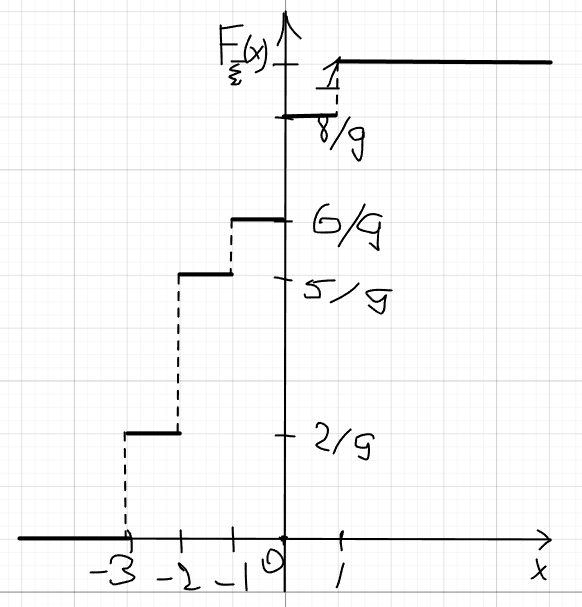
\includegraphics[width=0.5\linewidth]{2idz_1.png}
    \caption{}
\end{figure}
\begin{figure}[H]
    \centering
    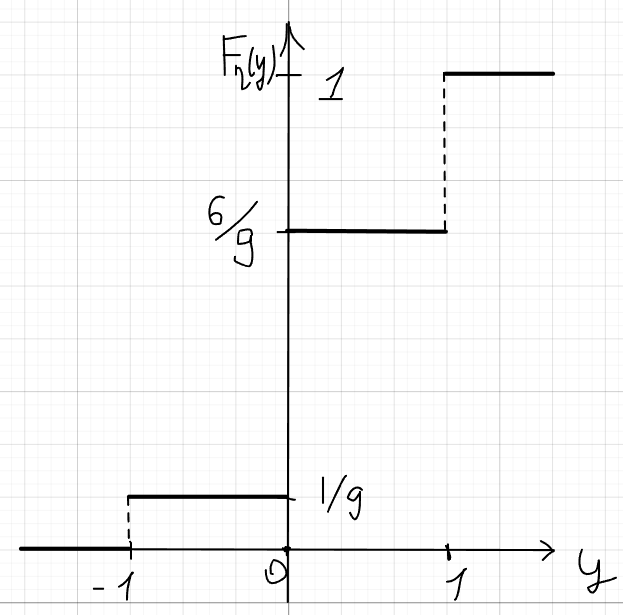
\includegraphics[width=0.5\linewidth]{2idz_2.png}
    \caption{}
\end{figure}

Ответ: $\Expect\xi$ = -1.3333, $\Variance\xi$ = 1.7778, $\Entropy\xi$ = 1.1887 нат\\

\end{proof}

%%%%%%%%%%%%%% ЗАДАНИЕ №2 %%%%%%%%%%%%%%
%% Условие задания №2
\begin{problem}
Дана плотность распределения абсолютно непрерывной случайной величины $\xi$:
\[ 
p_{\xi}(x) = \begin{cases} 
          C|x|, & x\in [\frac{-2\pi}{3}; 2\pi] \\
          0, & \text{в отс. сл.} \\
       \end{cases}
\]
Вычислить С, $\Expect\xi $, $\Variance\xi $, $\Entropy\xi $ (в натах). Вычислить распределение $\eta = \cos{\xi}$. Построить графики функций распределений $ F_{\xi}(x)$ и $ F_{\eta}(y)$.
\end{problem}

%% Решение задания №2
\begin{proof}
Найдем С:

$\int\limits_{-\infty}^{\infty}p_{\xi}(x)dx = C\int\limits_\frac{-2\pi}{3}^{2\pi}xdx = -C\int\limits_\frac{-2\pi}{3}^{0}xdx + C\int\limits_{0}^{2\pi}xdx = \frac{20\pi^2}{9}C = 1 \Rightarrow C = \frac{9}{20\pi^2}\\
$
И тогда:\\

$p_{\xi}(x) = \begin{cases} 
          \frac{9}{20\pi^2}|x|, & x\in [\frac{-2\pi}{3}; 2\pi] \\
          0, & \text{в отс. сл.} \\
       \end{cases}\\
$
Найдем мат. ожидание:\\
$
\Expect\xi = \int\limits_{-\infty}^{\infty}x\cdot p_{\xi}(x)dx =\int\limits_\frac{-2\pi}{3}^{2\pi}x\frac{9}{20\pi^2}|x|dx = \int\limits_\frac{-2\pi}{3}^\frac{2\pi}{3}x\frac{9}{20\pi^2}|x|dx + \int\limits_\frac{2\pi}{3}^{2\pi}x^2\frac{9}{20\pi^2}dx = 0 + \frac{52\pi}{45} \approx 3,6303\\
$
Найдем дисперсию:\\
$\Expect\xi^2 = \int\limits_{-\infty}^{\infty}x^2\cdot p_{\xi}(x)dx =\int\limits_\frac{-2\pi}{3}^{2\pi}x^2\frac{9}{20\pi^2}|x|dx = \int\limits_\frac{-2\pi}{3}^{0}x^2\frac{9}{20\pi^2}|x|dx + \int\limits_{0}^{2\pi}x^2\frac{9}{20\pi^2}|x|dx = \int\limits_{0}^{\frac{2\pi}{3}}x^3\frac{9}{20\pi^2}dx + \int\limits_{0}^{2\pi}x^3\frac{9}{20\pi^2}dx = \frac{82\pi^2}{45} \approx \\ \approx 17,9846\\$
$\Variance\xi = \Expect\xi^2 - (\Expect\xi)^2 = \frac{82\pi^2}{45} - \frac{2704\pi^2}{2025} = \frac{986\pi^2}{2025} \approx 4,8056\\$$

Найдем энтропию:\\

$\Entropy\xi = -\int\limits_{-\infty}^{\infty}p_{\xi}(x)\cdot\ln(p_{\xi}(x))dx = -\left(\int\limits_{\frac{-2\pi}{3}}^0-x\frac{9}{20\pi^2}\ln\frac{-9x}{20\pi^2}dx + \int\limits_0^{2\pi}\frac{9}{20\pi^2}x\ln\frac{9x}{20\pi^2}dx\right) \approx 1,8599 \text{нат}$\\

$\supp\xi = [\frac{-2\pi}{3};2\pi], \eta = \cos{\xi} \Rightarrow \supp\eta = [-1;1]$.\\
Поскольку функция не монотонна на промежутке $[\frac{-2\pi}{3};2\pi]$ разобьем его:
$\supp\xi = [\frac{-2\pi}{3};0] \cup [0;\pi] \cup [\pi;2\pi]$

\begin{figure}[H]
    \centering
    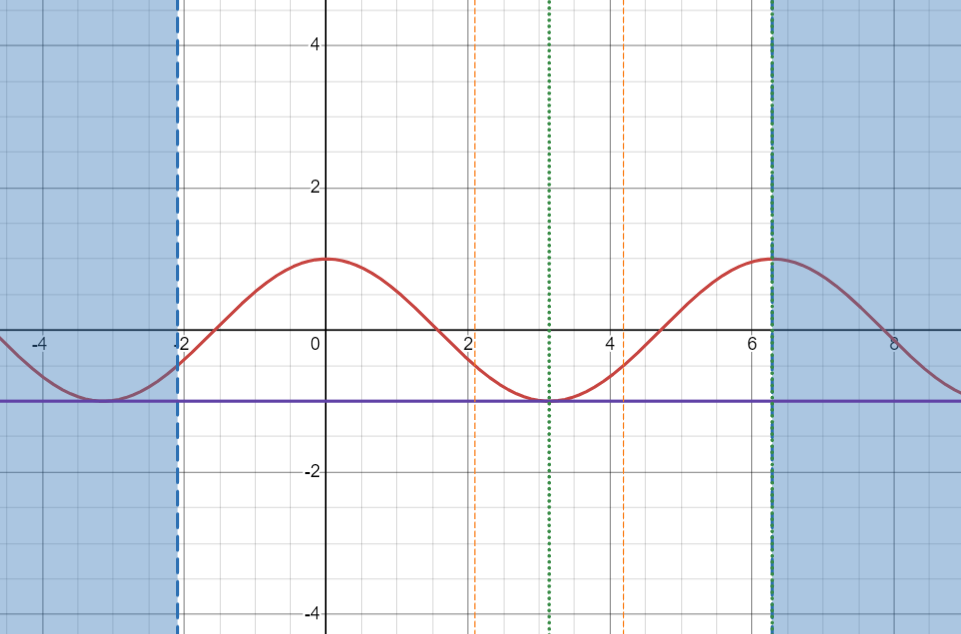
\includegraphics[width=0.5\linewidth]{2idz_3.png}
    \caption{}
\end{figure}
1) $\eta \in [-1;-\frac{1}{2}], \xi \in [\frac{2\pi}{3};\frac{4\pi}{3}]$\\
\[
A_{1,1} \in [\frac{2\pi}{3};\pi] \Rightarrow \begin{cases}
    g_{1,1}(x) = \cos{x}\\
    g_{1,1}^{-1}(y) = \arccos{y}\\
\end{cases}
\]
\[
A_{1,2} \in [\pi;\frac{4\pi}{3}] \Rightarrow \begin{cases}
    g_{1,2}(x) = \cos{x}\\
    g_{1,2}^{-1}(y) = 2\pi -\arccos{y}\\
\end{cases}
\]
$p_{1\eta}(y) = \frac{1}{\sqrt{1 - y^2}}\cdot \frac{9}{20\pi^2}\cdot\arccos{y} + \frac{1}{\sqrt{1 - y^2}}\cdot \frac{9}{20\pi^2}\cdot(2\pi - \arccos{y}) = \frac{1}{\sqrt{1 - y^2}}\cdot \frac{9 \cdot 2\pi}{20\pi^2}\\$

2) $\eta \in [-\frac{1}{2};0], \xi \in [-\frac{2\pi}{3};-\frac{\pi}{2}]\cup       [\frac{\pi}{2};\frac{2\pi}{3}] \cup [\frac{4\pi}{3};\frac{3\pi}{2}]$\\
\[
A_{2,1} \in [-\frac{2\pi}{3};-\frac{\pi}{2}] \Rightarrow \begin{cases}
    g_{2,1}(x) = \cos{x}\\
    g_{2,1}^{-1}(y) = -\arccos{y}\\
\end{cases}
\]
\[
A_{2,2} \in [\frac{\pi}{2};\frac{2\pi}{3}] \Rightarrow \begin{cases}
    g_{2,2}(x) = \cos{x}\\
    g_{2,2}^{-1}(y) = \arccos{y}\\
\end{cases}
\]
\[
A_{2,3} \in [\frac{4\pi}{3};\frac{3\pi}{2}] \Rightarrow \begin{cases}
    g_{2,3}(x) = \cos{x}\\
    g_{2,3}^{-1}(y) = 2\pi -\arccos{y}\\
\end{cases}
\]
$p_{2\eta}(y) = \frac{1}{\sqrt{1 - y^2}}\cdot\frac{9}{20\pi^2}\cdot\arccos{y} + \frac{1}{\sqrt{1 - y^2}}\cdot\frac{9}{20\pi^2}\cdot\arccos{y} + \frac{1}{\sqrt{1 - y^2}}\cdot\frac{9}{20\pi^2}\cdot(2\pi - \arccos{y}) = \frac{9\arccos{y} + 18\pi}{20\pi^2 \sqrt{1-y^2}}\\$

3) $\eta \in [0;1], \xi \in [-\frac{\pi}{2};0] \cup [0;\frac{\pi}{2}] \cup [\frac{3\pi}{2};2\pi]$\\
\[
A_{3,1} \in [-\frac{\pi}{2};0] \Rightarrow \begin{cases}
    g_{3,1}(x) = \cos{x}\\
    g_{3,1}^{-1}(y) = -\arccos{y}\\
\end{cases}
\]
\[
A_{3,2} \in [0;\frac{\pi}{2}] \Rightarrow \begin{cases}
    g_{3,2}(x) = \cos{x}\\
    g_{3,2}^{-1}(y) = \arccos{y}\\
\end{cases}
\]
\[
A_{3,3} \in [\frac{3\pi}{2};2\pi] \Rightarrow \begin{cases}
    g_{3,3}(x) = \cos{x}\\
    g_{3,3}^{-1}(y) = 2\pi -\arccos{y}\\
\end{cases}
\]
$p_{3\eta}(y) = \frac{1}{\sqrt{1 - y^2}}\cdot\frac{9}{20\pi^2}\cdot\arccos{y} + \frac{1}{\sqrt{1 - y^2}}\cdot\frac{9}{20\pi^2}\cdot\arccos{y} + \frac{1}{\sqrt{1 - y^2}}\cdot\frac{9}{20\pi^2}\cdot(2\pi - \arccos{y}) = \frac{9\arccos{y} + 18\pi}{20\pi^2 \sqrt{1-y^2}}\\$

\[
p_{\eta}(y) = \begin{cases}
    \frac{1}{\sqrt{1 - y^2}}\cdot \frac{9 \cdot 2\pi}{20\pi^2}, & y\in [-1;-0,5]\\
   \frac{9\arccos{y} + 18\pi}{20\pi^2 \sqrt{1-y^2}}, & y\in [-0,5;1]\\
   0, & else\\
\end{cases}
\]

Найдем $ F_{\xi}(x)$ и $ F_{\eta}(y)$:

\[
F_{\xi}(x) = \int\limits_{-\infty}^xp_{\xi}(t)dt = \begin{cases}
    0, & x\in (-\infty;\frac{-2\pi}{3}]\\
    \frac{4\pi^2-9x^2}{40\pi^2}, & x\in (\frac{-2\pi}{3}; 0]\\
    \frac{4\pi^2+9x^2}{40\pi^2}, & x\in (0; 2\pi]\\
    1, & x\in (2\pi;+\infty)
\end{cases}
\]
\[
F_{\eta}(y) = \int\limits_{-\infty}^yp_{\eta}(t)dt = \begin{cases}
    0, & y\in (-\infty;-1]\\
    \frac{9\arcsin{y} + 4,5\pi}{10\pi}, & y\in (-1; -\frac{1}{2}]\\
    1 + \frac{-9(\arccos{y})^2 - 36\pi\arccos{y}}{40\pi^2}, & y\in (-\frac{1}{2}; 1]\\
    1, & y\in (1;\infty)
\end{cases}
\]
\begin{figure}[H]
    \centering
    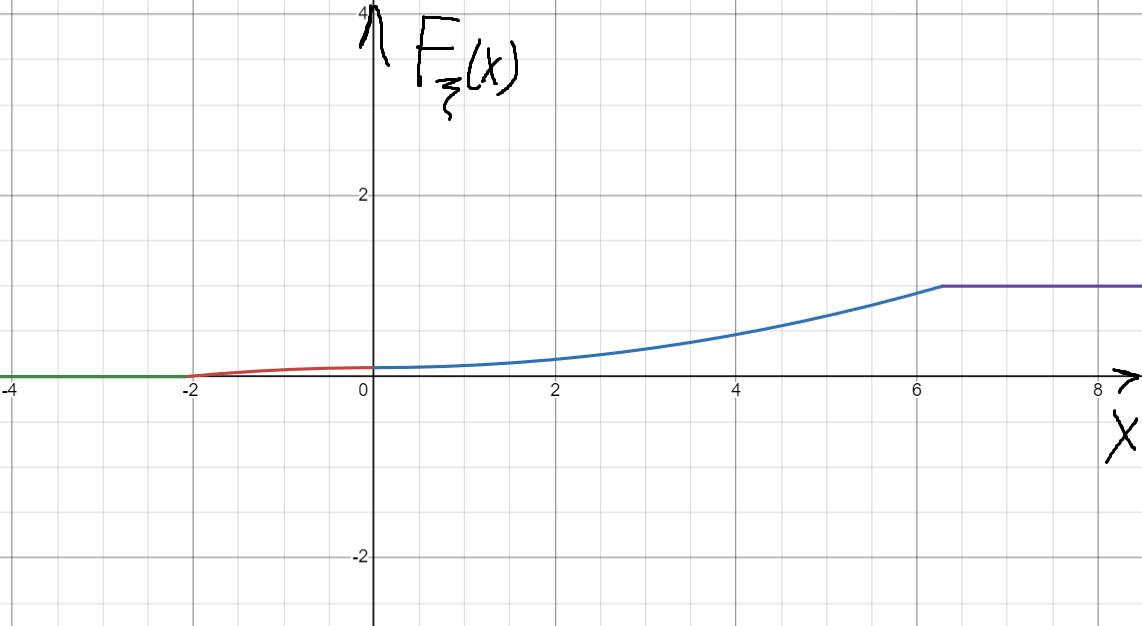
\includegraphics[width=0.5\linewidth]{2idz_4.png}
    \caption{}
\end{figure}
\begin{figure}[H]
    \centering
    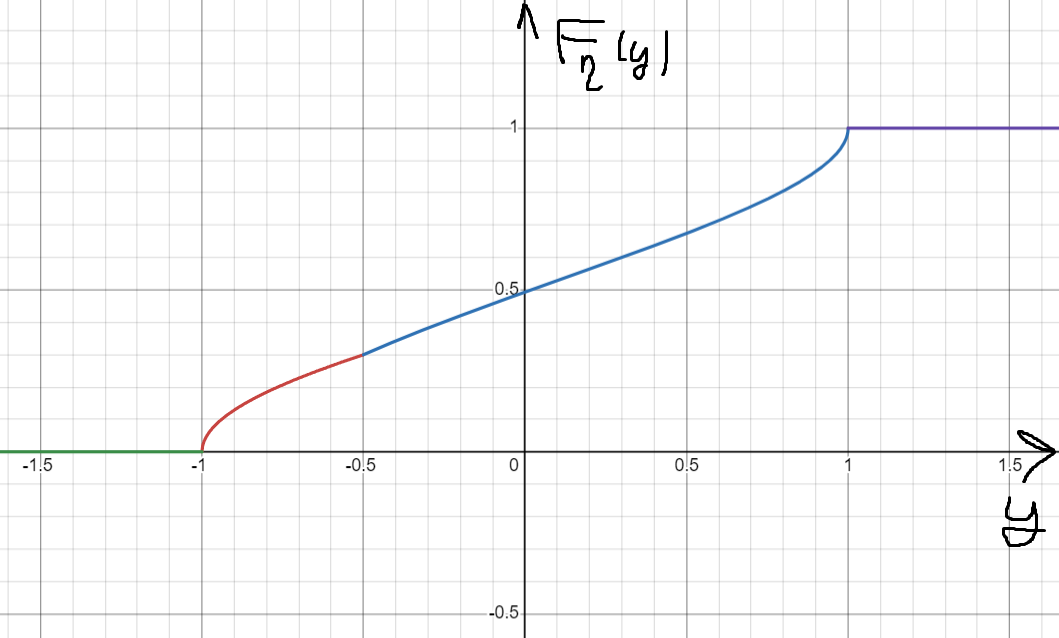
\includegraphics[width=0.5\linewidth]{2idz_5.png}
    \caption{}
\end{figure}\\
Ответ: $\Expect\xi$ = 3.6303, $\Variance\xi$ = 4.8056, $\Entropy\xi$ = 1.8599 нат\\
\end{proof}